% vim:ft=tex

\section{Prediction on Hourly Basis}
Just like in chapter \ref{sec:daily}, data prediction is performed with the MLP regressor again. This time, however, the granularity is refined at an hourly level. This makes more training data possible. Furthermore, new correlations are created between the individual features. However, this also requires some changes in the data preparation script. Up to this stage of the project, the aggregation level at day level was sufficient. To be able to format the data from a daily format into an hourly format, both the weather data of the DarkSky API and the cycling usage data have to be re-processed, which is described in more detail in section \ref{sec:dphourly}.
Since an hourly data prediction produces much more data than a daily prediction, this user story uses the built up Hadoop cluster as well as PySpark and Zeppelin. The tasks are typical tasks for a cluster-based calculation like Hadoop. Here, too, some parts are reused on the basis of previous scripts (e.g. the generated or calculated weather data).
section \ref{sec:learnpred} deals with the training and prediction of the regression model based on the hourly prepared usage data. Subsequently it is described how the data set can be extended by additional features like "Age" or "local Events". The acquisition of these additional data was carried out by Ankur Mehra project team. 
\subsection{Data Preparation}\label{sec:dphourly}
Since the long term goal was to predict the usage on a hourly base, some further data
transformation steps are necessary to achieve this goal. Furthermore the data records will
increase significantly on an hourly granularity. Therefore the normal use of Anaconda and Jupyter
on a local computer may be not sufficient due to low physical memory. An ideal use case for our
newly installed Hadoop cluster! There PySpark can be used as already used under Data Profiling
Part 1 in chapter \ref{dp1} to manage \glqq big data\grqq transformations. Unfortunately the behavior and syntax of PySpark
is sometimes a little more complicated than Pandas. For example, in PySpark it is not easily
possible to iterate over rows since the data frame is distributed over the worker nodes and thus it
only allows column wise operations. Moreover, Pandas operations such as „iloc“ are not available
in PySpark. But the API comes also with some advantages, e.g. it is quite performant on big data
scale (i.e. it can easily perform several million of records) and it has an SQL approach.
Functions like \glqq select\grqq \glqq where\grqq and \glqq filter\grqq are syntactical close by to SQL as we know from MySQL
and other database management systems.\\\\
The structure of the weather data is inconsistent due to "hourly weather"  While the other columns
only contain simple values, the column "hourly weather" contains nested JSON lists. This means
that these nested lists must somehow become normal columns. This was a little more complicated
than expected, but not impossible. Fortunately, PySpark allows one to define \glqq schemas\grqq that are
used as a kind of blueprint by Spark to read the Spark data frame. With the following code one
can already create normal columns from the JSON lists:
\begin{figure}[H]
\hspace{-1.6cm}
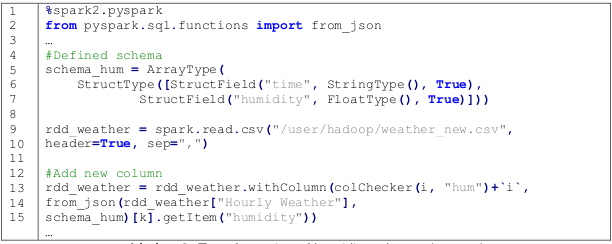
\includegraphics[width=1.2\textwidth]{img/listing5}\label{fig:listing5}
\captionof{figure}{Transformation of humidity columns (excerpt)}\label{fig:listing5}
\end{figure}
he excerpt from \ref{fig:listing5} shows that \glqq structTypes\grqq can be used to search the individual sub lists
of \glqq hourly weather\grqq .
The complete script is contained in the Zeppelin notebook \glqq DFGeneration.json\grqq and can also be found on GitHub.
\\\\
The described transformation creates a new column with the corresponding value for each hour.
The script works dynamically. For example, the user can look at the data with two hours from today,
which then looks like this:
\begin{figure}[H]
\hspace{-1.6cm}
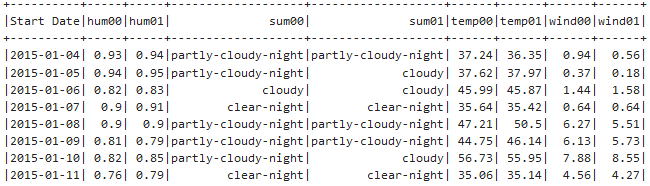
\includegraphics[width=1.2\textwidth]{img/figure7_weather_df}\label{fig:figure7_weather_df}
\captionof{figure}{Weather dataframe after transformation for two hours}\label{fig:figure7_weather_df}
\end{figure}
This (figure \ref{fig:figure7_weather_df}), however, is more like a jumping window technique as it uses days as start date
and not the the single hours on each day. Nevertheless the structure of the data frame from figure \ref{fig:figure7_weather_df} can be used as ground for applying sliding window method.\\\\
However, before the sliding window procedure could be implemented, the \glqq Start Date\grqq from figure \ref{fig:figure7_weather_df} had to be converted to an hourly format, whereby the individual hour columns had to be
combined so that only one \glqq current column\grqq existed. For example, \glqq hum00\grqq and \glqq hum01\grqq should
become something like \glqq Current Humidity\grqq  which shows the humidity value of each hour. This
means that further data preparation steps are necessary.\\\\
First, the exact timestamps of the bicycle data were read in from the provided TfL website and
rounded off to an hourly level. For example, \glqq 23:38\grqq became \glqq 23:00\grqq  Minutes and seconds were
ignored. An arithmetic lap (half-round mode) did not make sense, because then there would be
overlaps with the successor day when 23 o'clock is rounded up. However, this also means that a
slight distortion must be assumed. For example, many bicycles could be rented at a bicycle station
at 17:52 and significantly less after 18 o'clock. Then one would notice a peak at 17 o'clock and a
low usage at 18 o'clock, although in fact more bicycles were rented around 18 o'clock.\\\\
Another problem was that not for every hour there was data about the usage of the bicycle stations.
However, this data quality problem could be solved relatively easy. The missing hours can be
determined by a user defined function. Since every day has 24 hours, this can be calculated
manually as following (figure \ref{fig:listing6}):
\begin{figure}[H]
\hspace{-1.6cm}
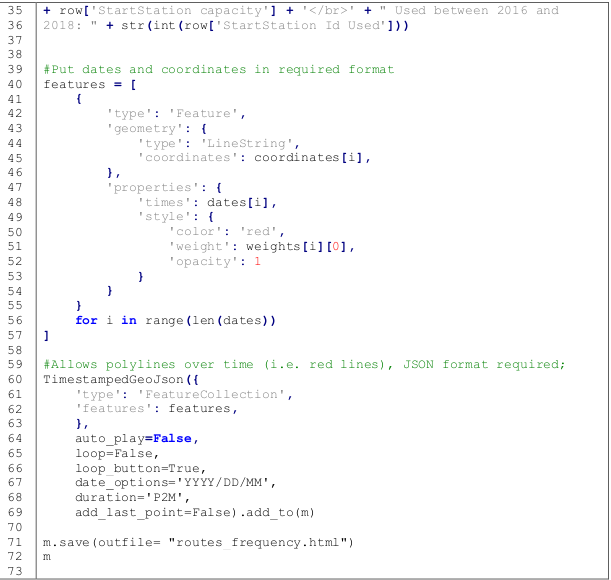
\includegraphics[width=1.2\textwidth]{img/listing2}\label{fig:listing6}
\captionof{figure}{Adding missing hours on usage data}\label{fig:listing6}
\end{figure}
A prerequisite of this method from figure \ref{fig:listing6} is that at least one maximum value and one minimum
value exist that serve as boundaries. If no data was collected on a day at a station, null values
would appear. This does not happen, however, and even if it did, it would be removed at a later
stage as such data does not provide any advantage for training a machine learning model.\\\\
Another problem was how to transform the individual hour columns of the weather data so that
only one column exists instead of e.g. 24 columns, whereby this new column should contain all
values of the 24 columns arranged correctly. Fortunately the function \glqq explode\grqq exists in PySpark
and is provided via the class \glqq pyspark.sql.functions\grqq  With \glqq explode\grqq an array can be passed,
which then returns a new line for each element of the array \cite{RN8}. The corresponding code excerpt
looks as following:
\begin{figure}[H]
\hspace{-1.6cm}
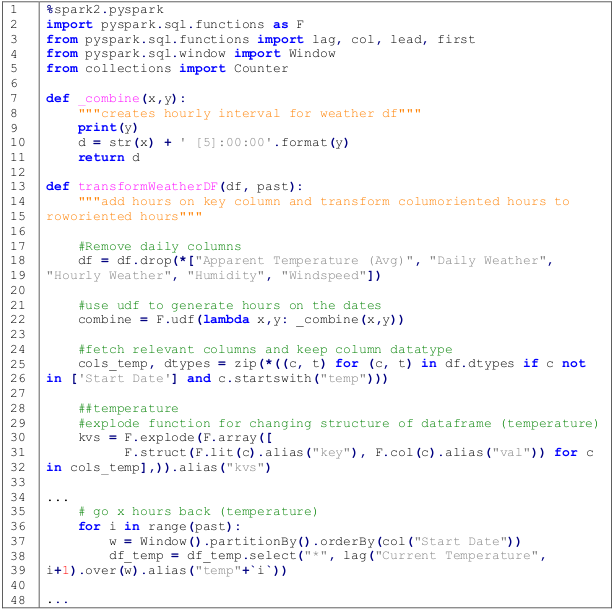
\includegraphics[width=1.2\textwidth]{img/listing7}\label{fig:listing7}
\captionof{figure}{Further transformation of weather data (excerpt)}\label{fig:listing7}
\end{figure}
The code example from figure \ref{fig:listing7} is used to transform the temperature columns, which are
combined into a single column as described above. Thus the weather data frame is prepared to
the extent that every hour of a day belongs to a specific hourly weather value. The lines 35 - 39 show the use of the PySpark function \glqq lag\grqq ,  that over a selected \glqq window\grqq takes the starting
boundary \cite{RN8}. If one increments the index at this point, he will get the previous value from the
window. Depending on how far one wants to go into the past, the window is moved over the data
set and thus a sliding window is achieved. This can also be adapted for the future. With the function
\glqq lead\grqq the ending boundary of a \glqq window\grqq is retrieved \cite{RN8}. Again, the future sliding window is only
applied for the usage (target variable) and not for the weather data or other columns.\\\\
The prepared hourly temperature data with sliding window looks finally as following:
\begin{figure}[H]
\centering
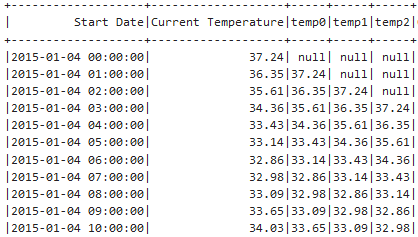
\includegraphics[width=0.8\textwidth]{img/figure8_temperature_df}\label{fig:figure8_temperature_df}
\captionof{figure}{Temperature dataframe after transformation for 3 hours (past)}\label{fig:figure8_temperature_df}
\end{figure}
In this example from figure \ref{fig:figure8_temperature_df} it is clearly recognizable that the initial values contain \glqq null\grqq values, which is due to the fact that no weather data was available before 04.01.2015 (or at least they
were not fetched from Dark Sky). The number of zero values increases with the number of selected
hours into the past. The same applies to the last lines of the Spark data frame, where null values
may be appear for the \glqq future usage\grqq columns. Therefore the first 20 and the last 20 lines of the
data frame are removed at the end.\\\\
With the described PySpark transformations it was possible to create dynamic hourly data frames,
which can then be used in the next step of the modeling phase. A corresponding test file can be
found on GitHub in the folder data preparation.
\subsubsection{Holidays}

To add the bank holidays are day-based, so they should be set on a 24 hour windows.
However, fixing the bank holidays from midnight to midnight the next day might not
be the best solution as people might consider the evening of a bank holiday the same
way as they do for normal week day, while the evening of the day before will be more
interesting. Indeed, when people want to go out in the evening and go to bed late,
they will prefer doing that when they don't have to wake up early in the morning,
thus they may be more likely to use a bike the end of the day before the bank
holiday than of the day itself.

This is why it might be a good idea to test the accuracy of the prediction
placing bank holidays from 6pm the day before to 6pm the day itself.

\subsection{Learning and Prediction}\label{sec:learnpred}

For the learning part, we used the same algorithm as described in~\ref{data_prediction}.
We trained twenty-four models, one per future hour to predict.
For each model, we only use the past and current data which we match to
the future expected number of rented bike for the given following hour,
no other future data is used.

We used the sliding-windows hourly based data over 48 hours (aggregating per slice
of 6 hours after the first 24 hours).
We have an accuracy of 0.800638 on the test dataset.
On the graph below, you can see several randomly selected days in the testing set
starting at midnight and predicting for the whole day. The title above each graph
indicates the date displayed, the actual expected value is in red and the
predicted one is in blue.
\begin{figure}[H]
\hspace{-0.9cm}
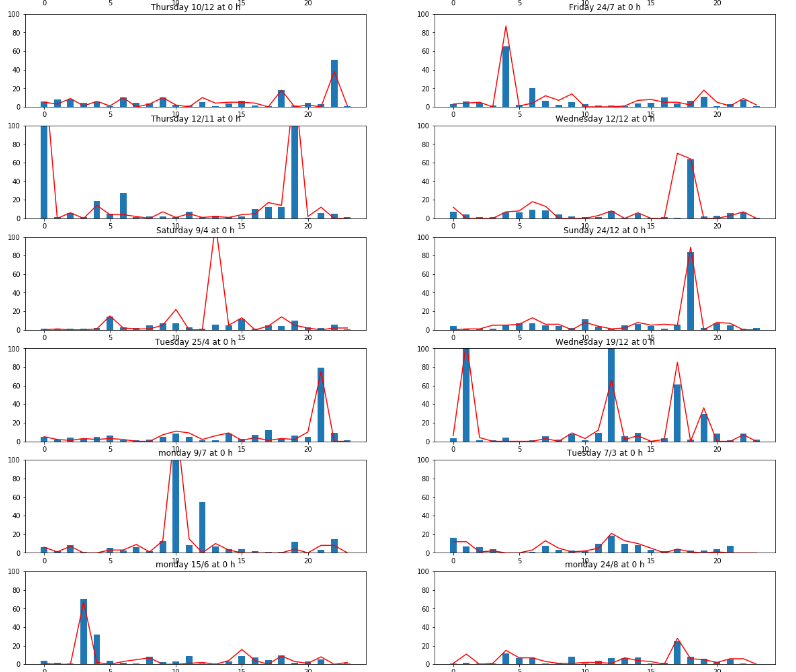
\includegraphics[width=1.1\textwidth]{img/hourly_predictions}
\captionof{figure}{Comparison of expected (red) and predicted (blue) hourly rented bikes on test dataset}\label{fig:hourly_pred}
\end{figure}

As we can see on the Figure~\ref{fig:hourly_pred} and considering the measured accuracy,
we can see that we can predict quite well the amount of rented bikes for the following
24 hours based on the data of the previous 48 hours.
